\documentclass{article}
\usepackage{graphicx}
\usepackage{tikz}
\usepackage{pgfplots}
\usepgfplotslibrary{groupplots}

%\usepackage[a4paper,bindingoffset=0.2in,left=1in,right=1in,top=1in,bottom=1in,footskip=.25in]{geometry}
\usepackage[export]{adjustbox}
\usepackage{xcolor}
\usepackage{mdframed}
\mdfdefinestyle{mdstyle}{align=center,innertopmargin=2pt,
    innerleftmargin=1pt,innerrightmargin=0pt,innerbottommargin=2pt,backgroundcolor=gray!50,linecolor=gray!50}
\definecolor{gray}{RGB}{220,220,220}
\pagenumbering{gobble}
\tikzset{style={inner sep=0,outer sep=0}}
\pgfplotsset{compat=1.17,
	yticklabel style = {/pgf/number format/assume math mode=true, font = {\fontsize{10pt}{12pt}\fontfamily{cmss} \selectfont}},
	x tick label style = {font= {\fontsize{12pt}{12pt} \fontfamily{qcr} \selectfont}},
	legend style = {font = {\fontsize{12pt}{12pt} \fontfamily{qcr} \selectfont}},
	title style = {font = {\fontsize{14pt}{14pt} \fontfamily{cmss} \selectfont}},
	xlabel style={yshift=-.3em},
	ylabel style={yshift=.2em, font = {\fontsize{12pt}{12pt}\fontfamily{cmss} \selectfont}},
	every axis plot/.append style={very thick},
	axis line style = {ultra thick},
}

\begin{document}
\nopagecolor
\begin{mdframed}[style=mdstyle]
    \resizebox{\textwidth}{!}{
		% This file was created by tikzplotlib v0.9.9.
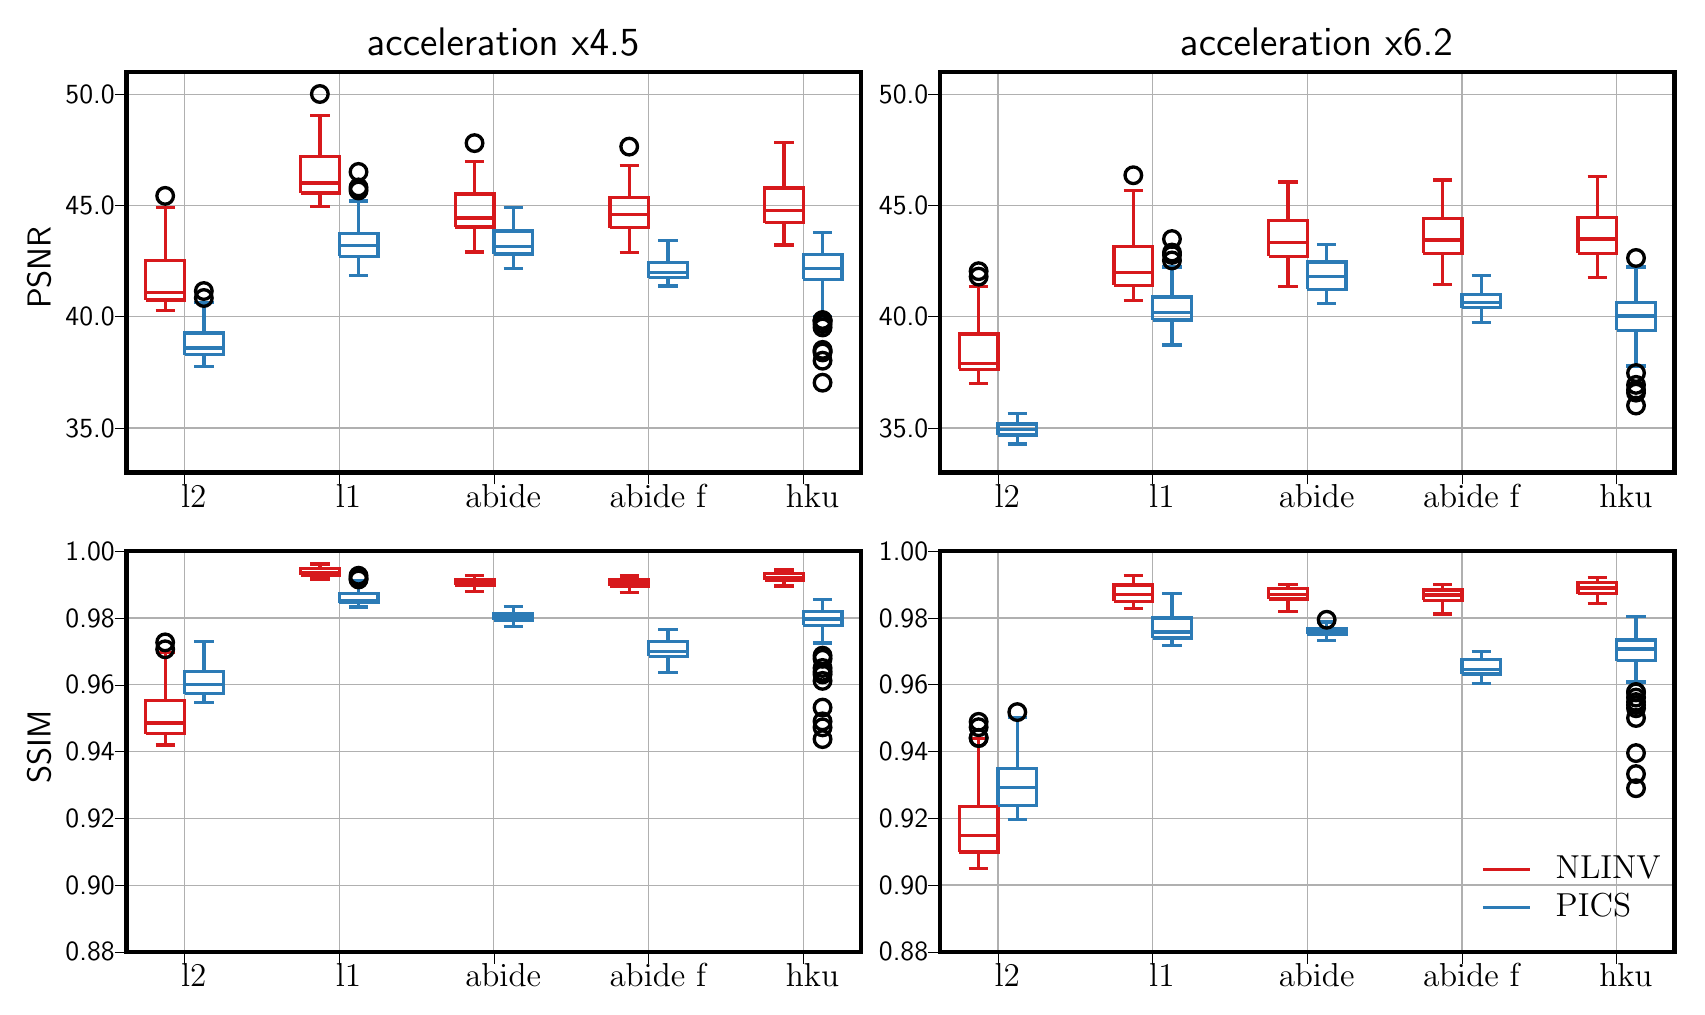
\begin{tikzpicture}

\definecolor{color0}{rgb}{0.843137254901961,0.0980392156862745,0.109803921568627}
\definecolor{color1}{rgb}{0.172549019607843,0.482352941176471,0.713725490196078}

\begin{groupplot}[group style={group size=2 by 2},width=0.9\textwidth, height=0.55\textwidth]
\nextgroupplot[
tick align=outside,
tick pos=left,
title={acceleration x4.5},
x grid style={white!69.0196078431373!black},
xmajorgrids,
xmin=-0.75, xmax=8.75,
xtick style={color=black},
xtick={0,2,4,6,8},
xticklabels={l2,l1,abide,abide f,hku},
y grid style={white!69.0196078431373!black},
ylabel={PSNR},
ymajorgrids,
ymin=33, ymax=51,
ytick style={color=black},
yticklabel style={/pgf/number format/.cd,fixed,fixed zerofill,precision=1},
]
\addplot [color0]
table {%
-0.5 40.7533224052753
0 40.7533224052753
0 42.5150633714072
-0.5 42.5150633714072
-0.5 40.7533224052753
};
\addplot [color0]
table {%
-0.25 40.7533224052753
-0.25 40.2914157637864
};
\addplot [color0]
table {%
-0.25 42.5150633714072
-0.25 44.9118432417704
};
\addplot [color0]
table {%
-0.375 40.2914157637864
-0.125 40.2914157637864
};
\addplot [color0]
table {%
-0.375 44.9118432417704
-0.125 44.9118432417704
};
\addplot [black, mark=o, mark size=3, mark options={solid,fill opacity=0}, only marks]
table {%
-0.25 45.4311084890718
};
\addplot [color0]
table {%
1.5 45.564405026352
2 45.564405026352
2 47.2074275749761
1.5 47.2074275749761
1.5 45.564405026352
};
\addplot [color0]
table {%
1.75 45.564405026352
1.75 44.9433972104571
};
\addplot [color0]
table {%
1.75 47.2074275749761
1.75 49.0369485681163
};
\addplot [color0]
table {%
1.625 44.9433972104571
1.875 44.9433972104571
};
\addplot [color0]
table {%
1.625 49.0369485681163
1.875 49.0369485681163
};
\addplot [black, mark=o, mark size=3, mark options={solid,fill opacity=0}, only marks]
table {%
1.75 50.0093882621187
};
\addplot [color0]
table {%
3.5 44.0297904159463
4 44.0297904159463
4 45.5172827213834
3.5 45.5172827213834
3.5 44.0297904159463
};
\addplot [color0]
table {%
3.75 44.0297904159463
3.75 42.9084970752752
};
\addplot [color0]
table {%
3.75 45.5172827213834
3.75 46.9753905814657
};
\addplot [color0]
table {%
3.625 42.9084970752752
3.875 42.9084970752752
};
\addplot [color0]
table {%
3.625 46.9753905814657
3.875 46.9753905814657
};
\addplot [black, mark=o, mark size=3, mark options={solid,fill opacity=0}, only marks]
table {%
3.75 47.8025425285198
};
\addplot [color0]
table {%
5.5 43.9992186969818
6 43.9992186969818
6 45.3585556309406
5.5 45.3585556309406
5.5 43.9992186969818
};
\addplot [color0]
table {%
5.75 43.9992186969818
5.75 42.8901136333959
};
\addplot [color0]
table {%
5.75 45.3585556309406
5.75 46.785941927504
};
\addplot [color0]
table {%
5.625 42.8901136333959
5.875 42.8901136333959
};
\addplot [color0]
table {%
5.625 46.785941927504
5.875 46.785941927504
};
\addplot [black, mark=o, mark size=3, mark options={solid,fill opacity=0}, only marks]
table {%
5.75 47.6442493058976
};
\addplot [color0]
table {%
7.5 44.2316852647214
8 44.2316852647214
8 45.7864667127963
7.5 45.7864667127963
7.5 44.2316852647214
};
\addplot [color0]
table {%
7.75 44.2316852647214
7.75 43.2270766279861
};
\addplot [color0]
table {%
7.75 45.7864667127963
7.75 47.8358051002919
};
\addplot [color0]
table {%
7.625 43.2270766279861
7.875 43.2270766279861
};
\addplot [color0]
table {%
7.625 47.8358051002919
7.875 47.8358051002919
};
\addplot [color1]
table {%
0 38.2944695466277
0.5 38.2944695466277
0.5 39.27295751767
0 39.27295751767
0 38.2944695466277
};
\addplot [color1]
table {%
0.25 38.2944695466277
0.25 37.7685561116441
};
\addplot [color1]
table {%
0.25 39.27295751767
0.25 40.6358639926393
};
\addplot [color1]
table {%
0.125 37.7685561116441
0.375 37.7685561116441
};
\addplot [color1]
table {%
0.125 40.6358639926393
0.375 40.6358639926393
};
\addplot [black, mark=o, mark size=3, mark options={solid,fill opacity=0}, only marks]
table {%
0.25 40.8426339617656
0.25 41.1557781639571
};
\addplot [color1]
table {%
2 42.7176922654106
2.5 42.7176922654106
2.5 43.7309901473682
2 43.7309901473682
2 42.7176922654106
};
\addplot [color1]
table {%
2.25 42.7176922654106
2.25 41.8624667283641
};
\addplot [color1]
table {%
2.25 43.7309901473682
2.25 45.1987567727012
};
\addplot [color1]
table {%
2.125 41.8624667283641
2.375 41.8624667283641
};
\addplot [color1]
table {%
2.125 45.1987567727012
2.375 45.1987567727012
};
\addplot [black, mark=o, mark size=3, mark options={solid,fill opacity=0}, only marks]
table {%
2.25 46.5079302529537
2.25 45.6736832542563
2.25 45.8117465005903
};
\addplot [color1]
table {%
4 42.8168671185658
4.5 42.8168671185658
4.5 43.8543126733638
4 43.8543126733638
4 42.8168671185658
};
\addplot [color1]
table {%
4.25 42.8168671185658
4.25 42.1740816682337
};
\addplot [color1]
table {%
4.25 43.8543126733638
4.25 44.8985500649015
};
\addplot [color1]
table {%
4.125 42.1740816682337
4.375 42.1740816682337
};
\addplot [color1]
table {%
4.125 44.8985500649015
4.375 44.8985500649015
};
\addplot [color1]
table {%
6 41.7541999813795
6.5 41.7541999813795
6.5 42.4347443785853
6 42.4347443785853
6 41.7541999813795
};
\addplot [color1]
table {%
6.25 41.7541999813795
6.25 41.3786047986911
};
\addplot [color1]
table {%
6.25 42.4347443785853
6.25 43.4226307515636
};
\addplot [color1]
table {%
6.125 41.3786047986911
6.375 41.3786047986911
};
\addplot [color1]
table {%
6.125 43.4226307515636
6.375 43.4226307515636
};
\addplot [color1]
table {%
8 41.6880476873872
8.5 41.6880476873872
8.5 42.8110827462093
8 42.8110827462093
8 41.6880476873872
};
\addplot [color1]
table {%
8.25 41.6880476873872
8.25 40.0122609607629
};
\addplot [color1]
table {%
8.25 42.8110827462093
8.25 43.7843577595792
};
\addplot [color1]
table {%
8.125 40.0122609607629
8.375 40.0122609607629
};
\addplot [color1]
table {%
8.125 43.7843577595792
8.375 43.7843577595792
};
\addplot [black, mark=o, mark size=3, mark options={solid,fill opacity=0}, only marks]
table {%
8.25 39.5190307956185
8.25 38.3956912470801
8.25 37.0368028976554
8.25 39.8226797801844
8.25 38.5104572946682
8.25 39.6663383318749
8.25 38.0252563949126
8.25 39.8526960525653
8.25 38.4507370681284
8.25 39.802496482388
};
\addplot [color0]
table {%
-0.5 41.0954349331529
0 41.0954349331529
};
\addplot [color0]
table {%
1.5 46.0042435489611
2 46.0042435489611
};
\addplot [color0]
table {%
3.5 44.4432667280331
4 44.4432667280331
};
\addplot [color0]
table {%
5.5 44.5938719201258
6 44.5938719201258
};
\addplot [color0]
table {%
7.5 44.7736622094884
8 44.7736622094884
};
\addplot [color1]
table {%
0 38.5954480600655
0.5 38.5954480600655
};
\addplot [color1]
table {%
2 43.2061863937121
2.5 43.2061863937121
};
\addplot [color1]
table {%
4 43.1518341763932
4.5 43.1518341763932
};
\addplot [color1]
table {%
6 41.9981432318237
6.5 41.9981432318237
};
\addplot [color1]
table {%
8 42.1754635443622
8.5 42.1754635443622
};

\nextgroupplot[
tick align=outside,
tick pos=left,
title={acceleration x6.2},
x grid style={white!69.0196078431373!black},
xmajorgrids,
xmin=-0.75, xmax=8.75,
xtick style={color=black},
xtick={0,2,4,6,8},
xticklabels={l2,l1,abide,abide f,hku},
y grid style={white!69.0196078431373!black},
ymajorgrids,
ymin=33, ymax=51,
ytick style={color=black},
yticklabel style={/pgf/number format/.cd,fixed,fixed zerofill,precision=1},
]
\addplot [color0]
table {%
-0.5 37.6390990070379
0 37.6390990070379
0 39.2182512521342
-0.5 39.2182512521342
-0.5 37.6390990070379
};
\addplot [color0]
table {%
-0.25 37.6390990070379
-0.25 37.0154711278083
};
\addplot [color0]
table {%
-0.25 39.2182512521342
-0.25 41.3515828249506
};
\addplot [color0]
table {%
-0.375 37.0154711278083
-0.125 37.0154711278083
};
\addplot [color0]
table {%
-0.375 41.3515828249506
-0.125 41.3515828249506
};
\addplot [black, mark=o, mark size=3, mark options={solid,fill opacity=0}, only marks]
table {%
-0.25 42.0467204628729
-0.25 41.8027310941708
};
\addplot [color0]
table {%
1.5 41.4183535500363
2 41.4183535500363
2 43.1598687657176
1.5 43.1598687657176
1.5 41.4183535500363
};
\addplot [color0]
table {%
1.75 41.4183535500363
1.75 40.7441879670417
};
\addplot [color0]
table {%
1.75 43.1598687657176
1.75 45.6842489682423
};
\addplot [color0]
table {%
1.625 40.7441879670417
1.875 40.7441879670417
};
\addplot [color0]
table {%
1.625 45.6842489682423
1.875 45.6842489682423
};
\addplot [black, mark=o, mark size=3, mark options={solid,fill opacity=0}, only marks]
table {%
1.75 46.3578595819879
};
\addplot [color0]
table {%
3.5 42.7204763291901
4 42.7204763291901
4 44.3170038683143
3.5 44.3170038683143
3.5 42.7204763291901
};
\addplot [color0]
table {%
3.75 42.7204763291901
3.75 41.3564640060385
};
\addplot [color0]
table {%
3.75 44.3170038683143
3.75 46.0589521438599
};
\addplot [color0]
table {%
3.625 41.3564640060385
3.875 41.3564640060385
};
\addplot [color0]
table {%
3.625 46.0589521438599
3.875 46.0589521438599
};
\addplot [color0]
table {%
5.5 42.8435002025296
6 42.8435002025296
6 44.4055168469634
5.5 44.4055168469634
5.5 42.8435002025296
};
\addplot [color0]
table {%
5.75 42.8435002025296
5.75 41.4372425483763
};
\addplot [color0]
table {%
5.75 44.4055168469634
5.75 46.1447429738825
};
\addplot [color0]
table {%
5.625 41.4372425483763
5.875 41.4372425483763
};
\addplot [color0]
table {%
5.625 46.1447429738825
5.875 46.1447429738825
};
\addplot [color0]
table {%
7.5 42.8473556346941
8 42.8473556346941
8 44.4685020090034
7.5 44.4685020090034
7.5 42.8473556346941
};
\addplot [color0]
table {%
7.75 42.8473556346941
7.75 41.7550565759475
};
\addplot [color0]
table {%
7.75 44.4685020090034
7.75 46.3067684733337
};
\addplot [color0]
table {%
7.625 41.7550565759475
7.875 41.7550565759475
};
\addplot [color0]
table {%
7.625 46.3067684733337
7.875 46.3067684733337
};
\addplot [color1]
table {%
0 34.6855875446927
0.5 34.6855875446927
0.5 35.1825707809999
0 35.1825707809999
0 34.6855875446927
};
\addplot [color1]
table {%
0.25 34.6855875446927
0.25 34.2863934747273
};
\addplot [color1]
table {%
0.25 35.1825707809999
0.25 35.6470085495676
};
\addplot [color1]
table {%
0.125 34.2863934747273
0.375 34.2863934747273
};
\addplot [color1]
table {%
0.125 35.6470085495676
0.375 35.6470085495676
};
\addplot [color1]
table {%
2 39.8494091480339
2.5 39.8494091480339
2.5 40.8866743046603
2 40.8866743046603
2 39.8494091480339
};
\addplot [color1]
table {%
2.25 39.8494091480339
2.25 38.7328380317613
};
\addplot [color1]
table {%
2.25 40.8866743046603
2.25 42.229821851506
};
\addplot [color1]
table {%
2.125 38.7328380317613
2.375 38.7328380317613
};
\addplot [color1]
table {%
2.125 42.229821851506
2.375 42.229821851506
};
\addplot [black, mark=o, mark size=3, mark options={solid,fill opacity=0}, only marks]
table {%
2.25 43.4913400317912
2.25 42.7768598714846
2.25 42.8836588271234
2.25 42.5294684548173
};
\addplot [color1]
table {%
4 41.2255621087398
4.5 41.2255621087398
4.5 42.4561290415316
4 42.4561290415316
4 41.2255621087398
};
\addplot [color1]
table {%
4.25 41.2255621087398
4.25 40.6033169742786
};
\addplot [color1]
table {%
4.25 42.4561290415316
4.25 43.2532473957039
};
\addplot [color1]
table {%
4.125 40.6033169742786
4.375 40.6033169742786
};
\addplot [color1]
table {%
4.125 43.2532473957039
4.375 43.2532473957039
};
\addplot [color1]
table {%
6 40.4103236062831
6.5 40.4103236062831
6.5 41.0099787872403
6 41.0099787872403
6 40.4103236062831
};
\addplot [color1]
table {%
6.25 40.4103236062831
6.25 39.7304620390107
};
\addplot [color1]
table {%
6.25 41.0099787872403
6.25 41.8503241980099
};
\addplot [color1]
table {%
6.125 39.7304620390107
6.375 39.7304620390107
};
\addplot [color1]
table {%
6.125 41.8503241980099
6.375 41.8503241980099
};
\addplot [color1]
table {%
8 39.3841845997606
8.5 39.3841845997606
8.5 40.63235152665
8 40.63235152665
8 39.3841845997606
};
\addplot [color1]
table {%
8.25 39.3841845997606
8.25 37.7821899080596
};
\addplot [color1]
table {%
8.25 40.63235152665
8.25 42.2424621815717
};
\addplot [color1]
table {%
8.125 37.7821899080596
8.375 37.7821899080596
};
\addplot [color1]
table {%
8.125 42.2424621815717
8.375 42.2424621815717
};
\addplot [black, mark=o, mark size=3, mark options={solid,fill opacity=0}, only marks]
table {%
8.25 36.9388579133473
8.25 36.708491093456
8.25 36.5896676596521
8.25 36.0115813816048
8.25 37.4704743056059
8.25 42.6411398306153
};
\addplot [color0]
table {%
-0.5 37.9071078718664
0 37.9071078718664
};
\addplot [color0]
table {%
1.5 41.996537627121
2 41.996537627121
};
\addplot [color0]
table {%
3.5 43.3268854940329
4 43.3268854940329
};
\addplot [color0]
table {%
5.5 43.4530207992521
6 43.4530207992521
};
\addplot [color0]
table {%
7.5 43.4986445498824
8 43.4986445498824
};
\addplot [color1]
table {%
0 34.9462238233629
0.5 34.9462238233629
};
\addplot [color1]
table {%
2 40.2017359419396
2.5 40.2017359419396
};
\addplot [color1]
table {%
4 41.8119183114518
4.5 41.8119183114518
};
\addplot [color1]
table {%
6 40.6536335324146
6.5 40.6536335324146
};
\addplot [color1]
table {%
8 40.0289040287628
8.5 40.0289040287628
};

\nextgroupplot[
tick align=outside,
tick pos=left,
x grid style={white!69.0196078431373!black},
xmajorgrids,
xmin=-0.75, xmax=8.75,
xtick style={color=black},
xtick={0,2,4,6,8},
xticklabels={l2,l1,abide,abide f,hku},
y grid style={white!69.0196078431373!black},
ylabel={SSIM},
ymajorgrids,
ymin=0.88, ymax=1,
ytick style={color=black},
yticklabel style={/pgf/number format/.cd,fixed,fixed zerofill,precision=2}
]
\addplot [color0]
table {%
-0.5 0.945377861511377
0 0.945377861511377
0 0.955347955459671
-0.5 0.955347955459671
-0.5 0.945377861511377
};
\addplot [color0]
table {%
-0.25 0.945377861511377
-0.25 0.941951457711994
};
\addplot [color0]
table {%
-0.25 0.955347955459671
-0.25 0.969773598677379
};
\addplot [color0]
table {%
-0.375 0.941951457711994
-0.125 0.941951457711994
};
\addplot [color0]
table {%
-0.375 0.969773598677379
-0.125 0.969773598677379
};
\addplot [black, mark=o, mark size=3, mark options={solid,fill opacity=0}, only marks]
table {%
-0.25 0.972706105796683
-0.25 0.970634426669782
};
\addplot [color0]
table {%
1.5 0.992802086602753
2 0.992802086602753
2 0.994931044263125
1.5 0.994931044263125
1.5 0.992802086602753
};
\addplot [color0]
table {%
1.75 0.992802086602753
1.75 0.99172511115701
};
\addplot [color0]
table {%
1.75 0.994931044263125
1.75 0.996201458972811
};
\addplot [color0]
table {%
1.625 0.99172511115701
1.875 0.99172511115701
};
\addplot [color0]
table {%
1.625 0.996201458972811
1.875 0.996201458972811
};
\addplot [color0]
table {%
3.5 0.989844930609808
4 0.989844930609808
4 0.991615189554388
3.5 0.991615189554388
3.5 0.989844930609808
};
\addplot [color0]
table {%
3.75 0.989844930609808
3.75 0.987882009846365
};
\addplot [color0]
table {%
3.75 0.991615189554388
3.75 0.992729828037255
};
\addplot [color0]
table {%
3.625 0.987882009846365
3.875 0.987882009846365
};
\addplot [color0]
table {%
3.625 0.992729828037255
3.875 0.992729828037255
};
\addplot [color0]
table {%
5.5 0.989631273431831
6 0.989631273431831
6 0.991450749499421
5.5 0.991450749499421
5.5 0.989631273431831
};
\addplot [color0]
table {%
5.75 0.989631273431831
5.75 0.987553902804585
};
\addplot [color0]
table {%
5.75 0.991450749499421
5.75 0.992622958452653
};
\addplot [color0]
table {%
5.625 0.987553902804585
5.875 0.987553902804585
};
\addplot [color0]
table {%
5.625 0.992622958452653
5.875 0.992622958452653
};
\addplot [color0]
table {%
7.5 0.991383827536127
8 0.991383827536127
8 0.993329017359647
7.5 0.993329017359647
7.5 0.991383827536127
};
\addplot [color0]
table {%
7.75 0.991383827536127
7.75 0.989595915217068
};
\addplot [color0]
table {%
7.75 0.993329017359647
7.75 0.99435683537687
};
\addplot [color0]
table {%
7.625 0.989595915217068
7.875 0.989595915217068
};
\addplot [color0]
table {%
7.625 0.99435683537687
7.875 0.99435683537687
};
\addplot [color1]
table {%
0 0.957340812872022
0.5 0.957340812872022
0.5 0.964079288275555
0 0.964079288275555
0 0.957340812872022
};
\addplot [color1]
table {%
0.25 0.957340812872022
0.25 0.9547787739298
};
\addplot [color1]
table {%
0.25 0.964079288275555
0.25 0.97293703794648
};
\addplot [color1]
table {%
0.125 0.9547787739298
0.375 0.9547787739298
};
\addplot [color1]
table {%
0.125 0.97293703794648
0.375 0.97293703794648
};
\addplot [color1]
table {%
2 0.98461942108785
2.5 0.98461942108785
2.5 0.987321426408105
2 0.987321426408105
2 0.98461942108785
};
\addplot [color1]
table {%
2.25 0.98461942108785
2.25 0.983345315985918
};
\addplot [color1]
table {%
2.25 0.987321426408105
2.25 0.99106512858849
};
\addplot [color1]
table {%
2.125 0.983345315985918
2.375 0.983345315985918
};
\addplot [color1]
table {%
2.125 0.99106512858849
2.375 0.99106512858849
};
\addplot [black, mark=o, mark size=3, mark options={solid,fill opacity=0}, only marks]
table {%
2.25 0.99266924894617
2.25 0.991551293507814
2.25 0.991825116937606
};
\addplot [color1]
table {%
4 0.979326660849032
4.5 0.979326660849032
4.5 0.981163237910685
4 0.981163237910685
4 0.979326660849032
};
\addplot [color1]
table {%
4.25 0.979326660849032
4.25 0.977524946374716
};
\addplot [color1]
table {%
4.25 0.981163237910685
4.25 0.983436860231526
};
\addplot [color1]
table {%
4.125 0.977524946374716
4.375 0.977524946374716
};
\addplot [color1]
table {%
4.125 0.983436860231526
4.375 0.983436860231526
};
\addplot [color1]
table {%
6 0.968493896530638
6.5 0.968493896530638
6.5 0.973044037746791
6 0.973044037746791
6 0.968493896530638
};
\addplot [color1]
table {%
6.25 0.968493896530638
6.25 0.96360288192426
};
\addplot [color1]
table {%
6.25 0.973044037746791
6.25 0.976591947555143
};
\addplot [color1]
table {%
6.125 0.96360288192426
6.375 0.96360288192426
};
\addplot [color1]
table {%
6.125 0.976591947555143
6.375 0.976591947555143
};
\addplot [color1]
table {%
8 0.977816228369745
8.5 0.977816228369745
8.5 0.981971141969873
8 0.981971141969873
8 0.977816228369745
};
\addplot [color1]
table {%
8.25 0.977816228369745
8.25 0.972550079471324
};
\addplot [color1]
table {%
8.25 0.981971141969873
8.25 0.985562169187127
};
\addplot [color1]
table {%
8.125 0.972550079471324
8.375 0.972550079471324
};
\addplot [color1]
table {%
8.125 0.985562169187127
8.375 0.985562169187127
};
\addplot [black, mark=o, mark size=3, mark options={solid,fill opacity=0}, only marks]
table {%
8.25 0.961170521238044
8.25 0.947250584306902
8.25 0.965038652508318
8.25 0.967791547971193
8.25 0.953170577826649
8.25 0.968730271313922
8.25 0.963102352138443
8.25 0.963904037124977
8.25 0.943727293088123
8.25 0.949043446845677
};
\addplot [color0]
table {%
-0.5 0.948541740188323
0 0.948541740188323
};
\addplot [color0]
table {%
1.5 0.993695435018685
2 0.993695435018685
};
\addplot [color0]
table {%
3.5 0.990619988117553
4 0.990619988117553
};
\addplot [color0]
table {%
5.5 0.990524530185536
6 0.990524530185536
};
\addplot [color0]
table {%
7.5 0.992144321955469
8 0.992144321955469
};
\addplot [color1]
table {%
0 0.960166181556622
0.5 0.960166181556622
};
\addplot [color1]
table {%
2 0.985330290037096
2.5 0.985330290037096
};
\addplot [color1]
table {%
4 0.980311916832721
4.5 0.980311916832721
};
\addplot [color1]
table {%
6 0.969952194237116
6.5 0.969952194237116
};
\addplot [color1]
table {%
8 0.979718719625237
8.5 0.979718719625237
};

\nextgroupplot[
legend cell align={left},
legend style={
  fill opacity=0,
  draw opacity=1,
  text opacity=1,
  at={(1,0.05)},
  anchor=south east,
  draw=none,
  fill=none
},
tick align=outside,
tick pos=left,
x grid style={white!69.0196078431373!black},
xmajorgrids,
xmin=-0.75, xmax=8.75,
xtick style={color=black},
xtick={0,2,4,6,8},
xticklabels={l2,l1,abide,abide f,hku},
y grid style={white!69.0196078431373!black},
ymajorgrids,
ymin=0.88, ymax=1,
ytick style={color=black},
yticklabel style={/pgf/number format/.cd,fixed,fixed zerofill,precision=2}
]
\addplot [color0, forget plot]
table {%
-0.5 0.909917476135675
0 0.909917476135675
0 0.923540446716288
-0.5 0.923540446716288
-0.5 0.909917476135675
};
\addplot [color0, forget plot]
table {%
-0.25 0.909917476135675
-0.25 0.904976653964968
};
\addplot [color0, forget plot]
table {%
-0.25 0.923540446716288
-0.25 0.943869404048633
};
\addplot [color0, forget plot]
table {%
-0.375 0.904976653964968
-0.125 0.904976653964968
};
\addplot [color0, forget plot]
table {%
-0.375 0.943869404048633
-0.125 0.943869404048633
};
\addplot [black, mark=o, mark size=3, mark options={solid,fill opacity=0}, only marks, forget plot]
table {%
-0.25 0.948895000007803
-0.25 0.947282550100654
-0.25 0.944102117247453
-0.25 0.944030912825967
};
\addplot [color0, forget plot]
table {%
1.5 0.984980230188028
2 0.984980230188028
2 0.989927708553787
1.5 0.989927708553787
1.5 0.984980230188028
};
\addplot [color0, forget plot]
table {%
1.75 0.984980230188028
1.75 0.982847152641786
};
\addplot [color0, forget plot]
table {%
1.75 0.989927708553787
1.75 0.992711524126465
};
\addplot [color0, forget plot]
table {%
1.625 0.982847152641786
1.875 0.982847152641786
};
\addplot [color0, forget plot]
table {%
1.625 0.992711524126465
1.875 0.992711524126465
};
\addplot [color0, forget plot]
table {%
3.5 0.985645739790439
4 0.985645739790439
4 0.988740748297989
3.5 0.988740748297989
3.5 0.985645739790439
};
\addplot [color0, forget plot]
table {%
3.75 0.985645739790439
3.75 0.981942425548794
};
\addplot [color0, forget plot]
table {%
3.75 0.988740748297989
3.75 0.989944855695613
};
\addplot [color0, forget plot]
table {%
3.625 0.981942425548794
3.875 0.981942425548794
};
\addplot [color0, forget plot]
table {%
3.625 0.989944855695613
3.875 0.989944855695613
};
\addplot [color0, forget plot]
table {%
5.5 0.985286933854322
6 0.985286933854322
6 0.988421941866214
5.5 0.988421941866214
5.5 0.985286933854322
};
\addplot [color0, forget plot]
table {%
5.75 0.985286933854322
5.75 0.981163778076569
};
\addplot [color0, forget plot]
table {%
5.75 0.988421941866214
5.75 0.990005175823181
};
\addplot [color0, forget plot]
table {%
5.625 0.981163778076569
5.875 0.981163778076569
};
\addplot [color0, forget plot]
table {%
5.625 0.990005175823181
5.875 0.990005175823181
};
\addplot [color0, forget plot]
table {%
7.5 0.987300205610343
8 0.987300205610343
8 0.990587921261952
7.5 0.990587921261952
7.5 0.987300205610343
};
\addplot [color0, forget plot]
table {%
7.75 0.987300205610343
7.75 0.984357181197484
};
\addplot [color0, forget plot]
table {%
7.75 0.990587921261952
7.75 0.992229583647589
};
\addplot [color0, forget plot]
table {%
7.625 0.984357181197484
7.875 0.984357181197484
};
\addplot [color0, forget plot]
table {%
7.625 0.992229583647589
7.875 0.992229583647589
};
\addplot [color1, forget plot]
table {%
0 0.923839128344283
0.5 0.923839128344283
0.5 0.934838904192784
0 0.934838904192784
0 0.923839128344283
};
\addplot [color1, forget plot]
table {%
0.25 0.923839128344283
0.25 0.919715473158688
};
\addplot [color1, forget plot]
table {%
0.25 0.934838904192784
0.25 0.950176805910453
};
\addplot [color1, forget plot]
table {%
0.125 0.919715473158688
0.375 0.919715473158688
};
\addplot [color1, forget plot]
table {%
0.125 0.950176805910453
0.375 0.950176805910453
};
\addplot [black, mark=o, mark size=3, mark options={solid,fill opacity=0}, only marks, forget plot]
table {%
0.25 0.951809567786329
};
\addplot [color1, forget plot]
table {%
2 0.973999044394733
2.5 0.973999044394733
2.5 0.980005551047248
2 0.980005551047248
2 0.973999044394733
};
\addplot [color1, forget plot]
table {%
2.25 0.973999044394733
2.25 0.971810791132417
};
\addplot [color1, forget plot]
table {%
2.25 0.980005551047248
2.25 0.987435054715107
};
\addplot [color1, forget plot]
table {%
2.125 0.971810791132417
2.375 0.971810791132417
};
\addplot [color1, forget plot]
table {%
2.125 0.987435054715107
2.375 0.987435054715107
};
\addplot [color1, forget plot]
table {%
4 0.975215164571215
4.5 0.975215164571215
4.5 0.976783182080746
4 0.976783182080746
4 0.975215164571215
};
\addplot [color1, forget plot]
table {%
4.25 0.975215164571215
4.25 0.973315266372068
};
\addplot [color1, forget plot]
table {%
4.25 0.976783182080746
4.25 0.978783576986968
};
\addplot [color1, forget plot]
table {%
4.125 0.973315266372068
4.375 0.973315266372068
};
\addplot [color1, forget plot]
table {%
4.125 0.978783576986968
4.375 0.978783576986968
};
\addplot [black, mark=o, mark size=3, mark options={solid,fill opacity=0}, only marks, forget plot]
table {%
4.25 0.979469895123953
};
\addplot [color1, forget plot]
table {%
6 0.963193299974358
6.5 0.963193299974358
6.5 0.967643335693233
6 0.967643335693233
6 0.963193299974358
};
\addplot [color1, forget plot]
table {%
6.25 0.963193299974358
6.25 0.960283782303415
};
\addplot [color1, forget plot]
table {%
6.25 0.967643335693233
6.25 0.969945687204408
};
\addplot [color1, forget plot]
table {%
6.125 0.960283782303415
6.375 0.960283782303415
};
\addplot [color1, forget plot]
table {%
6.125 0.969945687204408
6.375 0.969945687204408
};
\addplot [color1, forget plot]
table {%
8 0.967239646000378
8.5 0.967239646000378
8.5 0.973374772766597
8 0.973374772766597
8 0.967239646000378
};
\addplot [color1, forget plot]
table {%
8.25 0.967239646000378
8.25 0.960833872346771
};
\addplot [color1, forget plot]
table {%
8.25 0.973374772766597
8.25 0.980373952262542
};
\addplot [color1, forget plot]
table {%
8.125 0.960833872346771
8.375 0.960833872346771
};
\addplot [color1, forget plot]
table {%
8.125 0.980373952262542
8.375 0.980373952262542
};
\addplot [black, mark=o, mark size=3, mark options={solid,fill opacity=0}, only marks, forget plot]
table {%
8.25 0.954810017415353
8.25 0.939531203498603
8.25 0.952959453473925
8.25 0.929005631531359
8.25 0.95390879156917
8.25 0.957830210932285
8.25 0.933242070778285
8.25 0.950045160544683
8.25 0.957718631183773
8.25 0.956163687291013
};
\addplot [very thick, color0]
table {%
0 0
};
\addlegendentry{NLINV}
\addplot [very thick, color1]
table {%
0 0
};
\addlegendentry{PICS}
\addplot [color0, forget plot]
table {%
-0.5 0.914793895946051
0 0.914793895946051
};
\addplot [color0, forget plot]
table {%
1.5 0.986955072000874
2 0.986955072000874
};
\addplot [color0, forget plot]
table {%
3.5 0.987023675969439
4 0.987023675969439
};
\addplot [color0, forget plot]
table {%
5.5 0.986927480461036
6 0.986927480461036
};
\addplot [color0, forget plot]
table {%
7.5 0.988980331912138
8 0.988980331912138
};
\addplot [color1, forget plot]
table {%
0 0.929287662321545
0.5 0.929287662321545
};
\addplot [color1, forget plot]
table {%
2 0.975813985151465
2.5 0.975813985151465
};
\addplot [color1, forget plot]
table {%
4 0.975867978501655
4.5 0.975867978501655
};
\addplot [color1, forget plot]
table {%
6 0.964606982933973
6.5 0.964606982933973
};
\addplot [color1, forget plot]
table {%
8 0.970732169042715
8.5 0.970732169042715
};
\end{groupplot}

\end{tikzpicture}

}
\end{mdframed}

\end{document}
